\section{Participants and the two kinds of
work}\label{participants-and-the-two-kinds-of-work}

Miners register signed service endpoints and capabilities and retain
their models. Customers buy detection and transformation jobs through
separately quoted offers. Validators evaluate subnet-owned
benchmark tasks and submit weights. Benchmark curators maintain
permitted source material, production records, and hidden evaluation
labels. A customer-facing gateway may relay ciphertext, but receives no
decryption key.

Benchmark operator and coordinator denote administrative duties assigned
to named curators and validators before each round: funding and managing
the round, recording protocol-derived assignments, and obtaining baseline evidence. A pilot may
combine these duties in one service. The task owner is the customer for
private inference and the curator for a benchmark. Authorized evaluators
and auditors are assigned validators; judges, readers, and authorized
reviewers perform independent review for those validators. Automated
judges require the qualification described in
Section~\ref{preservation-before-revision-rewards}. The settlement adapter
is the proposed contract software for customer escrow and alpha
transfers, described in
Section~\ref{paid-asynchronous-jobs-and-on-chain-coordination}.

\par\medskip\noindent
\begin{tabularx}{\linewidth}{@{}LLL@{}}
\toprule
Property & Customer inference & Subnet benchmark \\
\midrule
Purpose & Serve a customer's request & Measure miners for emissions \\
Launch services & A: detection; B: transformation & A: detection;
B: transformation \\
Source of text & Customer & Authorized benchmark collection \\
Default input recipients & Customer and assigned miner & Curator,
assigned service miners, validators, commissioned reviewers \\
Evaluation & Customer acceptance & Fixed scoring policy and independent
review \\
Pangram submission & Excluded from the confidential job protocol &
Required for evasion tasks \\
Payment & Customer's quoted fee & Performance-dependent emissions \\
Training reuse & No automatic reuse & Only under the collection's
release terms \\
\bottomrule
\end{tabularx}
\par\medskip

\begin{figure}[H]
\centering
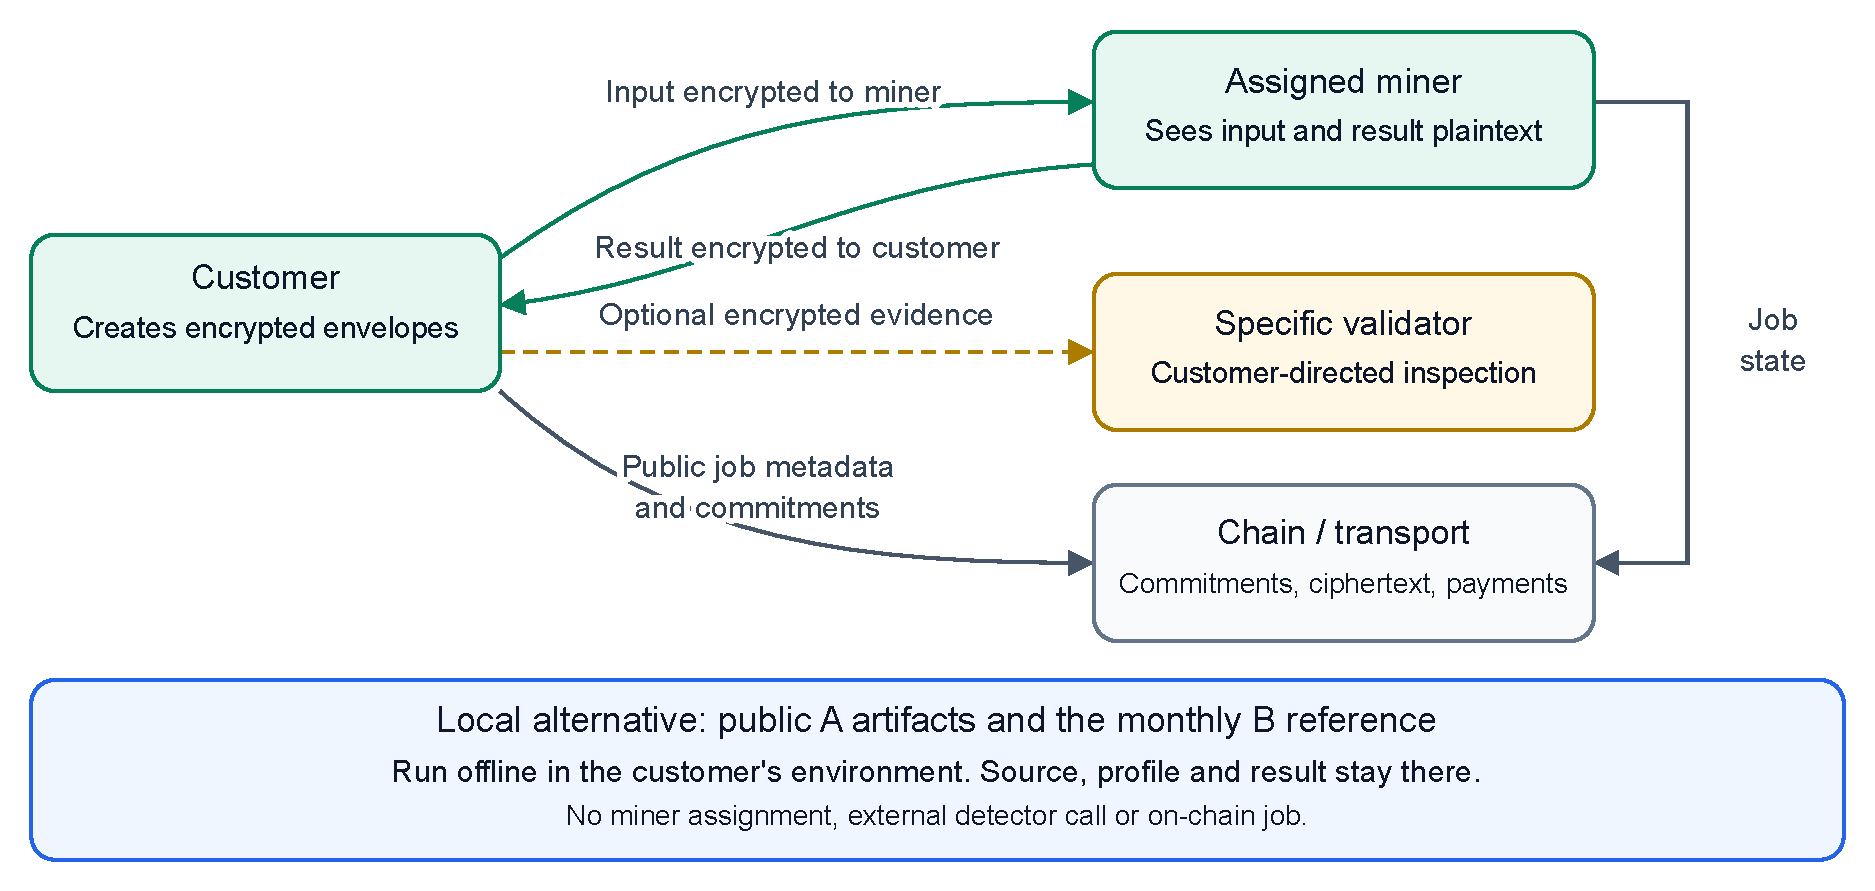
\includegraphics[width=\linewidth]{figures/private-inference.pdf}
\caption{Customer inference and optional evidence disclosure. Only the
addressed recipient can decrypt each envelope; endpoint handling remains
a trust assumption.}
\end{figure}

Customer tasks do not become benchmark examples automatically.
Validators must not obtain customer inputs through an audit exception, a
shared support key, or an arbitration process. A customer may initiate a
separate, explicitly addressed evidence disclosure as described in
Section~\ref{customer-directed-evidence-disclosure}. This applies to both
detection and transformation requests. An author's uploaded reference collection can be more identifying
than the query itself and receives the same protection.

Miners may advertise specialties, prices, length limits, and delivery
times. The network evaluates their observable service performance. It
cannot infer how many GPU hours they used, whether they own every
component, or which private weights produced a response. Emissions
create an incentive to improve training; they do not reimburse
unverifiable training claims.
